\title{\textbf{UnifiedRoPE: A Portable Rotary Position Embedding Attention Module for Multi-Architecture Transformers}}

\author{Anonymous authors}



\section{Introduction}

\subsection{Motivation}

\textbf{Rotary Position Embedding (RoPE)} (Su et al., 2021) encodes position 
information by rotating query and key vectors by position-dependent angles. 
It has become the default position encoding in modern decoder-only models:

\begin{itemize}
\item \textbf{LLaMA} (Touvron et al., 2023) -- RoPE
\item \textbf{Qwen} (Bai et al., 2023) -- RoPE
\item \textbf{Mistral} (Jiang et al., 2023) -- RoPE
\item \textbf{Gemma} (Mesnard et al., 2024) -- RoPE

\end{itemize}
RoPE offers three advantages over absolute position embeddings:

\begin{enumerate}
\item \textbf{Relative position encoding.} Attention scores depend only on
  $\Delta = i - j$, not on absolute positions.
\item \textbf{Length generalization.} RoPE extrapolates better to unseen sequence
  lengths.
\item \textbf{No learned parameters.} The rotation matrices are precomputed.

\end{enumerate}
However, porting RoPE-based attention to other architectures is 
non-trivial because:

\begin{itemize}
\item \textbf{DistilBERT} uses absolute position embeddings and flat attention
  (no nested structure).
\item \textbf{RoBERTa/BERT} use nested encoder attention where the output
  projection lives outside the inner attention.
\item \textbf{GPT-2} uses fused Conv1D with weights stored in \texttt{(in, out)} order.
\item \textbf{Qwen/LLaMA} use GQA, requiring KV head expansion.

\end{itemize}
Each architecture has its own quirks. A naive RoPE port breaks correctness 
on some of them.

\subsection{Problem Statement}

Given a pretrained transformer $\mathcal{M}$ from any of four families, we 
seek a \textbf{single attention module} $\mathcal{A}$ that:

\begin{enumerate}
\item Implements scaled dot-product attention with RoPE.
\item Correctly handles the architecture's conventions (nested, Conv1D, GQA).
\item Preserves base weights, producing identical output to the original
  attention.
\item Supports LoRA adapters for downstream fine-tuning.

\end{enumerate}
\subsection{Our Approach: UnifiedRoPE}

\textbf{UnifiedRoPE} is a single \texttt{nn.Module} that implements RoPE-based 
attention and works across four architecture families. Key design choices:

\begin{enumerate}
\item \textbf{Precomputed \texttt{cos}/\texttt{sin} caches.} RoPE frequencies are precomputed up
  to \texttt{max\_seq\_len} and stored as non-persistent buffers.

\item \textbf{Two RoPE entry points.} \texttt{\_apply\_rope} uses cached frequencies;
  \texttt{apply\_rotary\_pos\_emb} accepts externally-supplied \texttt{(cos, sin)} for
  compatibility with HuggingFace models that provide their own RoPE cache.

\item \textbf{Robust weight transfer.} \texttt{copy\_weights} handles 5 patterns:
\end{enumerate}
\begin{itemize}
\item GPT-2 fused \texttt{c\_attn} + \texttt{c\_proj}
\item RoBERTa nested \texttt{self.query/key/value} + \texttt{output.dense}
\item Qwen flat \texttt{q\_proj/k\_proj/v\_proj/o\_proj}
\item DistilBERT flat \texttt{q\_lin/k\_lin/v\_lin/out\_lin}
\item UniversalAdapter fallback

\end{itemize}
\begin{enumerate}
\item \textbf{LoRA preservation.} If the source module has LoRA adapters, they
  are preserved via \texttt{\_copy\_layer}.

\item \textbf{Nested encoder bypass.} RoBERTa's \texttt{output.dense} is outside the inner
  attention; UnifiedRoPE returns raw context and lets the outer layer
  project.

\item \textbf{GQA support.} \texttt{repeat\_kv} expands KV heads during forward.

\end{enumerate}
\subsection{UnifiedRoPE is Not a Compression Method}

\textbf{Important.} UnifiedRoPE does \textbf{not} reduce:
\begin{itemize}
\item Parameter count
\item KV-cache size
\item Attention compute

\end{itemize}
It is a \textbf{replacement module} that produces the same output as the 
original attention. Its purpose is to serve as a \textbf{substrate} for other 
compression techniques (LoRA recovery, SVD factorization, Nystr m 
approximation, MLA compression).

We emphasize this because the module is registered with the same registry 
as compression methods, but it does not itself compress.

\subsection{Contributions}

\begin{itemize}
\item \textbf{A single RoPE attention module} working across four architecture
  families without modification.
\item \textbf{A robust \texttt{copy\_weights}} handling GPT-2 Conv1D, RoBERTa nested
  encoder, Qwen GQA, and DistilBERT flat attention.
\item \textbf{LoRA preservation} during weight transfer.
\item \textbf{Precomputed RoPE caches} with non-persistent buffers.
\item \textbf{Full reproducibility.} Code and checkpoints released under
  Apache 2.0.

\end{itemize}
\subsection{Paper Organization}

Section 2 reviews related work. Section 3 provides background on RoPE and 
attention. Section 4 presents UnifiedRoPE. Section 5 describes 
architecture integration. Section 6 details the setup. Section 7 reports 
results. Section 8 analyzes portability. Section 9 discusses guidance. 
Section 10 lists limitations. Section 11 concludes.



\subsection{Notation}

\begin{lstlisting}

---
\end{lstlisting}


\section{Related Work}

\subsection{Position Embeddings in Transformers}

\subsubsection{Absolute Position Embeddings}

Vaswani et al. (2017) proposed learned absolute position embeddings. Used 
in GPT-1, BERT, RoBERTa, DistilBERT. Simple but do not generalize beyond 
trained lengths.

\subsubsection{Sinusoidal Position Embeddings}

Vaswani et al. (2017) also proposed fixed sinusoidal embeddings. Used in 
early transformers. Inferior to learned embeddings in practice.

\subsubsection{Relative Position Embeddings}

Shaw et al. (2018) introduced relative position embeddings conditioned on 
$\Delta = i - j$. T5 (Raffel et al., 2020) uses relative position biases.

\subsubsection{Rotary Position Embeddings (RoPE)}

Su et al. (2021) rotate $Q, K$ by position-dependent angles:

\[
\tilde{q}_i = q_i \cos(\theta_i) + \mathrm{rot}(q_i) \sin(\theta_i)
\tag{2.1}
\]

The resulting attention score depends only on $\Delta$. RoPE is now 
standard in LLaMA, Qwen, Mistral, and Gemma.

\subsubsection{ALiBi}

Press et al. (2022) use a linear bias instead of position embeddings. 
Alternative to RoPE.

\subsection{Attention Variants}

\subsubsection{Standard MHSA}

Vaswani et al. (2017). Four projections: $W_Q, W_K, W_V, W_O$.

\subsubsection{Multi-Query Attention (MQA)}

Shazeer (2019). Single KV head shared across queries.

\subsubsection{Grouped-Query Attention (GQA)}

Ainslie et al. (2023). $H_{kv} < H$ KV heads, repeated $H / H_{kv}$ times.

\subsubsection{Multi-Head Latent Attention (MLA)}

DeepSeek-AI (2024). Shared latent for K, V.

\subsection{Portability and Reproducibility}

\subsubsection{FlashAttention}

Dao et al. (2022) provide exact attention with IO-awareness. Ported to 
multiple GPUs.

\subsubsection{Reproducibility Studies}

Chen et al. (2024) reproduce FlashAttention. Wang et al. (2024) reproduce 
Performer. Our work is in the same spirit: we provide a portable RoPE 
attention and document the portability challenges.

\subsection{Position of Our Work}

\begin{table}[H]
\centering
\small
\begin{tabular}{lll}
\toprule
\textbf{Aspect} & \textbf{Su et al. 2021} & \textbf{This work} \\
\midrule
\textbf{RoPE formulation} & Novel & Reproduced \\
\textbf{Architecture support} & LLaMA & Four families \\
\textbf{Weight transfer} & Not addressed & Full support \\
\textbf{Nested encoder} & Not addressed & Explicit bypass \\
\textbf{Conv1D (GPT-2)} & Not addressed & Explicit transposition \\
\textbf{LoRA preservation} & Not addressed & Full support \\
\textbf{Purpose} & Novel method & Portability study \\
\bottomrule
\end{tabular}
\end{table}

\textbf{Key distinction.} UnifiedRoPE does not introduce a new position encoding. 
It provides a \textbf{single portable implementation} of RoPE attention that 
works across four families. The contribution is engineering, not science.
\begin{lstlisting}

---
\end{lstlisting}


\section{Background}

\subsection{Multi-Head Self-Attention}

For input $X \in \mathbb{R}^{B \times L \times d}$:

\[
\begin{aligned}
Q &= X W_Q, \quad K = X W_K, \quad V = X W_V \\
\text{head}_h &= \mathrm{softmax}\!\left(\frac{Q_h K_h^\top}{\sqrt{d_h}}\right) V_h \\
\text{MHSA}(X) &= \mathrm{Concat}(\text{head}_1, \dots, \text{head}_H) W_O
\end{aligned}
\tag{3.1}
\]

\subsection{Rotary Position Embedding (RoPE)}

RoPE encodes position by rotating each 2D subspace of $Q, K$:

\[
\tilde{q}_i = q_i \cos(\theta_i) + \mathrm{rot}(q_i) \sin(\theta_i)
\tag{3.2}
\]

where the rotation operator acts on the first half vs second half:

\[
\mathrm{rot}(x) = \begin{pmatrix} -x_{d_h/2:} \\ x_{:d_h/2} \end{pmatrix}
\tag{3.3}
\]

and $\theta_i$ is a position-dependent angle:

\[
\theta_i^{(k)} = i \cdot \omega_k, \qquad
\omega_k = \mathrm{base}^{-2k/d_h}, \quad k = 0, \dots, d_h/2 - 1
\tag{3.4}
\]

\textbf{Effect on attention.} The score between $q_i$ and $k_j$ depends only on 
$i - j$:

\[
\tilde{q}_i^\top \tilde{k}_j = f(q_i, k_j, i - j)
\tag{3.5}
\]

\subsection{Partial-Dimension RoPE}

Not all models apply RoPE to the full head dimension. For models with 
partial rotation (e.g., Qwen with \texttt{rotary\_dim < head\_dim}):

\[
\tilde{q}_i = \begin{pmatrix} q_i^{[:r]} \cos(\theta_i) + \mathrm{rot}(q_i^{[:r]}) \sin(\theta_i) \\ q_i^{[r:]} \end{pmatrix}
\tag{3.6}
\]

where $r$ is the rotary dimension. UnifiedRoPE supports this via 
\texttt{rotary\_dim = 2 * (head\_dim // 2)}.

\subsection{Grouped-Query Attention (GQA)}

$H_{kv} < H$ KV heads, repeated $H / H_{kv}$ times before attention:

\[
K_\text{expanded} = \mathrm{repeat\_kv}(K, H / H_{kv})
\tag{3.7}
\]

UnifiedRoPE applies \texttt{repeat\_kv} after RoPE.

\subsection{Nested Encoder Structure}

In BERT-style models:

\begin{lstlisting}
BertAttention
+-- self       (BertSelfAttention)
|   +-- query
|   +-- key
|   +-- value
+-- output     (BertSelfOutput)
    +-- dense  # $\leftarrow$ Output projection OUTSIDE
\end{lstlisting}

The output projection \texttt{output.dense} is \textbf{outside} the inner attention. 
When replacing the inner attention, the outer \texttt{output.dense} must still 
apply. UnifiedRoPE returns raw context and lets the outer layer project.

\subsection{Conv1D in GPT-2}

GPT-2 uses HuggingFace's \texttt{Conv1D}, which stores weights as \texttt{(in, out)}:

\begin{lstlisting}
class Conv1D(nn.Module):
    def __init__(self, nf, nx):
        self.weight = nn.Parameter(torch.empty(nx, nf))  # (in, out)
\end{lstlisting}

This is \textbf{transposed} relative to \texttt{nn.Linear}. UnifiedRoPE detects Conv1D 
and transposes during weight transfer.

\subsection{LoRA Adapters}

LoRA (Hu et al., 2021) adds trainable residuals:

\[
\Delta W = \frac{\alpha}{r} B A
\tag{3.8}
\]

with $B = 0$ at initialization. UnifiedRoPE's \texttt{LoRALinear} wraps this.

\subsection{Precomputed Caches}

RoPE angles $\theta_i$ are precomputed once:

\begin{lstlisting}
inv_freq = 1.0 / (base ** (arange(0, rotary_dim, 2) / rotary_dim))
t = arange(seq_len)
freqs = einsum("i,j->ij", t, inv_freq)
emb = cat([freqs, freqs], dim=-1)
cos_cached = emb.cos()
sin_cached = emb.sin()
\end{lstlisting}

UnifiedRoPE stores these as \textbf{non-persistent buffers} (\texttt{persistent=False}), 
so they are not saved with the model state dict.

\subsection{Notation Summary}

\begin{lstlisting}

---
\end{lstlisting}


\section{Method}

\subsection{Overview}

UnifiedRoPE implements RoPE-based scaled dot-product attention with a 
single \texttt{nn.Module}. It provides:

\begin{enumerate}
\item \textbf{LoRALinear projections} for Q, K, V, O.
\item \textbf{Precomputed RoPE caches} for fast frequency lookup.
\item \textbf{Robust weight transfer} across architectures.
\item \textbf{GQA expansion} via \texttt{repeat\_kv}.
\item \textbf{Nested encoder bypass} for RoBERTa-style models.

\end{enumerate}
\textbf{Figure 4.1} shows the pipeline.

\begin{lstlisting}
   +----------------------------------------------+
   |  Input X $\in$ R^{B $\times$ L $\times$ d}                     |
   +--------------------+-------------------------+
                        |
        +---------------+---------------+
                                         
   +---------+    +---------+    +---------+
   | q_proj  |    | k_proj  |    | v_proj  |
   | + LoRA  |    | + LoRA  |    | + LoRA  |
   +----+----+    +----+----+    +----+----+
        |              |              |
                                      |
   +---------+    +---------+         |
   | Apply   |    | Apply   |         |
   | RoPE    |    | RoPE    |         |
   +----+----+    +----+----+         |
        |              |              |
        |                             |
        |         +---------+         |
        |         | GQA     |         |
        |         | expand  |         |
        |         +----+----+         |
        |              |              |
        +------+-------+--------------+
                
        +--------------+
        |  Attention   |
        |  softmax(QK) |
        +------+-------+
               |
                
        +--------------+
        |  out_proj    |
        |  + LoRA      |
        +--------------+
\end{lstlisting}

\subsection{The `UnifiedRoPE` Module}

\subsubsection{Initialization}

\begin{lstlisting}
class UnifiedRoPE(BaseAttention):
    def __init__(self, config=None, rank=None, dim=None, num_heads=None,
                 max_seq_len=4096, base=10000, dropout=0.1,
                 pretrained_attn=None, lora_rank=16, lora_alpha=32.0,
                 is_decoder=None, **kwargs):
        # Resolve dimensions
        self.hidden_size = ...
        self.num_heads = ...
        self.num_kv_heads = ...
        self.head_dim = hidden_size // num_heads
        
        # LoRA projections
        self.q_proj = LoRALinear(hidden_size, q_head_size, lora_rank=..., freeze_base=True)
        self.k_proj = LoRALinear(hidden_size, kv_head_size, lora_rank=..., freeze_base=True)
        self.v_proj = LoRALinear(hidden_size, kv_head_size, lora_rank=..., freeze_base=True)
        self.out_proj = LoRALinear(q_head_size, hidden_size, lora_rank=..., freeze_base=True)
        
        # RoPE cache
        self.rotary_dim = 2 * (head_dim // 2)
        self.register_buffer("inv_freq", ..., persistent=False)
        self._build_cache(max_seq_len)
\end{lstlisting}

\subsubsection{Precomputed RoPE Cache}

\begin{lstlisting}
def _build_cache(self, seq_len):
    t = torch.arange(seq_len, dtype=self.inv_freq.dtype)
    freqs = torch.einsum("i,j->ij", t, self.inv_freq)
    emb = torch.cat((freqs, freqs), dim=-1)
    self.register_buffer("cos_cached", emb.cos(), persistent=False)
    self.register_buffer("sin_cached", emb.sin(), persistent=False)
\end{lstlisting}

\textbf{Note.} Buffers are \texttt{persistent=False}, so they are not stored in 
\texttt{state\_dict()}. This avoids checkpoint pollution.

\subsubsection{Applying RoPE}

\begin{lstlisting}
def _apply_rope(self, x, seq_len):
    rotary_dim = min(self.rotary_dim, self.cos_cached.shape[-1], x.shape[-1])
    rotary_dim = 2 * (rotary_dim // 2)
    
    cos = self.cos_cached[:seq_len, :rotary_dim].unsqueeze(0).unsqueeze(0)
    sin = self.sin_cached[:seq_len, :rotary_dim].unsqueeze(0).unsqueeze(0)
    
    if rotary_dim < x.shape[-1]:
        x_rot = x[..., :rotary_dim]
        x_pass = x[..., rotary_dim:]
        rotated = (x_rot * cos) + (_rotate_half(x_rot) * sin)
        return torch.cat((rotated, x_pass), dim=-1)
    else:
        return (x * cos) + (_rotate_half(x) * sin)
\end{lstlisting}

\subsection{Weight Transfer}

\subsubsection{Five Extraction Patterns}

UnifiedRoPE's \texttt{copy\_weights} handles:

\begin{table}[H]
\centering
\small
\begin{tabular}{lll}
\toprule
\textbf{Pattern} & \textbf{Architecture} & \textbf{Weights extracted} \\
\midrule
1 & GPT-2 & Split \texttt{c\_attn}; \texttt{c\_proj} for output \\
2 & RoBERTa & \texttt{self.query/key/value} + \texttt{output.dense} \\
3 & Qwen & \texttt{q\_proj/k\_proj/v\_proj/o\_proj} \\
4 & DistilBERT & \texttt{q\_lin/k\_lin/v\_lin/out\_lin} \\
5 & Fallback & UniversalAdapter \\
\bottomrule
\end{tabular}
\end{table}

\subsubsection{Conv1D Transposition}

\begin{lstlisting}
if c_attn_w.shape[0] == self.hidden_size and c_attn_w.shape[1] != self.hidden_size:
    c_attn_w = c_attn_w.t()
\end{lstlisting}

\subsubsection{Nested Encoder Detection}

\begin{lstlisting}
if hasattr(old_attn, "self") and hasattr(old_attn, "output"):
    self.is_nested_encoder = True
    src = old_attn.self
    if hasattr(old_attn.output, "dense"):
        w_o = old_attn.output.dense.weight
\end{lstlisting}

When nested, \texttt{out\_proj} is \textbf{skipped} in forward; the outer layer applies.

\subsubsection{LoRA Preservation}

The \texttt{\_copy\_layer} helper preserves source LoRA adapters:

\begin{lstlisting}
def _copy_layer(target_layer, w, b, src_sub=None):
    # Copy base weight
    if w is not None: ...
    # Copy bias
    if b is not None: ...
    # Preserve LoRA
    if src_sub is not None and hasattr(src_sub, "lora_A"):
        target_layer.lora_A.data.copy_(src_sub.lora_A.data)
        target_layer.lora_B.data.copy_(src_sub.lora_B.data)
\end{lstlisting}

\subsection{Forward Pass}

\begin{lstlisting}
def forward(self, hidden_states, attention_mask=None, ...):
    B, L, _ = hidden_states.shape
    
    # 1. Project
    q = self.q_proj(hidden_states).view(B, L, H, d_h).transpose(1, 2)
    k = self.k_proj(hidden_states).view(B, L, Hkv, d_h).transpose(1, 2)
    v = self.v_proj(hidden_states).view(B, L, Hkv, d_h).transpose(1, 2)
    
    # 2. Apply RoPE
    pos_emb = kwargs.get("position_embeddings")
    if pos_emb is not None:
        cos, sin = pos_emb
        q, k = apply_rotary_pos_emb(q, k, cos, sin)
    else:
        q = self._apply_rope(q, L)
        k = self._apply_rope(k, L)
    
    # 3. GQA expansion
    if self.num_kv_heads != self.num_heads:
        k = repeat_kv(k, self.num_key_value_groups)
        v = repeat_kv(v, self.num_key_value_groups)
    
    # 4. Scaled dot-product attention
    scores = q @ k^T / sqrt(d_h)
    
    # 5. Causal mask for decoders
    if self.is_decoder and L > 1:
        scores = scores + causal_mask
    
    # 6. Padding mask
    if attention_mask is not None:
        scores = apply_attention_mask(scores, attention_mask)
    
    # 7. Softmax, dropout, context
    attn = softmax(scores)
    context = attn @ v
    
    # 8. Output projection (skip if nested)
    if self.is_nested_encoder:
        output = context
    else:
        output = self.out_proj(context)
    
    return output, attn
\end{lstlisting}

\subsection{Two RoPE Entry Points}

\subsubsection{Internal `\_apply\_rope`}

Uses the cached \texttt{cos\_cached}, \texttt{sin\_cached} buffers. \textbf{Fast path} for models 
that do not supply their own RoPE cache.

\subsubsection{External `apply\_rotary\_pos\_emb`}

Accepts \texttt{(cos, sin)} from HuggingFace models that precompute their own 
RoPE. Used when \texttt{position\_embeddings} is passed in \texttt{forward}.

\textbf{Why two paths?} Some models (Qwen) supply their RoPE cache; others do 
not. UnifiedRoPE supports both.

\subsection{GQA Expansion}

For $H_{kv} < H$:

\begin{lstlisting}
if self.num_kv_heads != self.num_heads:
    k = repeat_kv(k, self.num_key_value_groups)
    v = repeat_kv(v, self.num_key_value_groups)
\end{lstlisting}

\texttt{repeat\_kv} broadcasts each KV head to \texttt{H / H\_{kv}} query heads.

\subsection{Nested Encoder Bypass}

For RoBERTa-style models:

\begin{lstlisting}
if self.is_nested_encoder:
    output = context   # Raw context
else:
    output = self.out_proj(context)
\end{lstlisting}

The outer \texttt{BertSelfOutput.dense} applies the projection.

\subsection{Complexity Analysis}

\begin{table}[H]
\centering
\small
\begin{tabular}{lll}
\toprule
\textbf{Phase} & \textbf{Time} & \textbf{Memory} \\
\midrule
Projections & $\mathcal{O}(L d^2)$ & $\mathcal{O}(L d)$ \\
RoPE application & $\mathcal{O}(L H d_h)$ & $\mathcal{O}(L H d_h)$ \\
GQA expansion & $\mathcal{O}(L H d_h)$ & $\mathcal{O}(L H d_h)$ \\
Attention & $\mathcal{O}(L^2 H d_h)$ & $\mathcal{O}(L^2 H)$ \\
Output projection & $\mathcal{O}(L d^2)$ & $\mathcal{O}(L d)$ \\
\textbf{Total} & $\mathcal{O}(L^2 H d_h + L d^2)$ & $\mathcal{O}(L^2 H + L d)$ \\
\bottomrule
\end{tabular}
\end{table}

\textbf{Same as standard attention.} No compression.

\subsection{Theoretical Notes}

\subsubsection{RoPE Rotation Correctness}

\textbf{Proposition.} The rotation operator preserves L2 norm:

\[
\|\tilde{q}_i\|_2 = \|q_i\|_2
\tag{4.1}
\]

\textbf{Proof.} Rotation matrices are orthogonal. $\square$

\subsubsection{Relative Position Property}

\textbf{Proposition.} The attention score satisfies:

\[
\tilde{q}_i^\top \tilde{k}_j = f(q_i, k_j, i - j)
\tag{4.2}
\]

\textbf{Proof.} Classical (Su et al., 2021). $\square$

\subsubsection{GQA Equivalence}

\textbf{Proposition.} GQA with \texttt{repeat\_kv} produces the same output as if the 
KV heads were duplicated.

\textbf{Proof.} \texttt{repeat\_kv} literally duplicates. $\square$

\subsection{Summary}

UnifiedRoPE:
\begin{enumerate}
\item Implements RoPE-based attention.
\item Works across four architectures.
\item Preserves base weights.
\item Supports LoRA.
\item \textbf{Does not compress.}

\end{enumerate}
It is a \textbf{substrate} for other compression techniques.
\begin{lstlisting}

---
\end{lstlisting}


\section{Architecture Integration}

\subsection{Model Support}

\begin{table}[H]
\centering
\small
\begin{tabular}{llllllll}
\toprule
\textbf{Model} & \textbf{Layers} & \textbf{$d$} & \textbf{$H$} & \textbf{$H_{kv}$} & \textbf{Nested?} & \textbf{Conv1D?} & \textbf{RoPE?} \\
\midrule
DistilBERT-base & 6 & 768 & 12 & 12 & No & No & \textbf{Added} \\
RoBERTa-base & 12 & 768 & 12 & 12 & Yes & No & \textbf{Added} \\
GPT-2 & 12 & 768 & 12 & 12 & No & Yes & \textbf{Added} \\
Qwen3.5-0.8B & 24 & 1024 & 8 & 2 & No & No & Native \\
\bottomrule
\end{tabular}
\end{table}

\textbf{Note.} DistilBERT, RoBERTa, and GPT-2 use absolute position embeddings. 
UnifiedRoPE \textbf{adds} RoPE on top, which may not match pretrained behavior.

For Qwen, RoPE is native -- UnifiedRoPE simply preserves it.

\subsection{DistilBERT (Flat)}

\begin{lstlisting}
distilbert.transformer.layer.0.attention
+-- q_lin  (Linear 768 $\to$ 768)
+-- k_lin  (Linear 768 $\to$ 768)
+-- v_lin  (Linear 768 $\to$ 768)
+-- out_lin (Linear 768 $\to$ 768)
\end{lstlisting}

\textbf{Weight extraction:}
\begin{lstlisting}
w_q = src.q_lin.weight.detach()
w_k = src.k_lin.weight.detach()
w_v = src.v_lin.weight.detach()
w_o = src.out_lin.weight.detach()
\end{lstlisting}

\texttt{is\_nested\_encoder = False}.

\textbf{RoPE caveat.} DistilBERT was trained with absolute positions. Adding 
RoPE changes the attention pattern. Accuracy may drop unless recovery 
fine-tuning adapts.

\subsection{RoBERTa (Nested)}

\begin{lstlisting}
roberta.encoder.layer.0.attention
+-- self
|   +-- query, key, value
+-- output
    +-- dense
\end{lstlisting}

\textbf{Nested detection:}
\begin{lstlisting}
if hasattr(old_attn, "self") and hasattr(old_attn, "output"):
    self.is_nested_encoder = True
    src = old_attn.self
    w_o = old_attn.output.dense.weight
\end{lstlisting}

\texttt{is\_nested\_encoder = True}. Forward returns raw context.

\subsection{GPT-2 (Causal Conv1D)}

\begin{lstlisting}
transformer.h.0.attn
+-- c_attn  (Conv1D 768 $\to$ 2304)
+-- c_proj  (Conv1D 768 $\to$ 768)
\end{lstlisting}

\textbf{Split c\_attn:}
\begin{lstlisting}
c_attn_w = src.c_attn.weight.detach()
if c_attn_w.shape[0] == self.hidden_size and c_attn_w.shape[1] != self.hidden_size:
    c_attn_w = c_attn_w.t()
q_dim = self.q_head_size
k_dim = self.kv_head_size
v_dim = self.kv_head_size
w_q = c_attn_w[:q_dim, :]
w_k = c_attn_w[q_dim:q_dim+k_dim, :]
w_v = c_attn_w[q_dim+k_dim:, :]
\end{lstlisting}

\texttt{is\_nested\_encoder = False}. Causal mask applied in forward.

\subsection{Qwen3.5 (GQA + RoPE)}

\begin{lstlisting}
model.layers.0.self_attn
+-- q_proj  (Linear 1024 $\to$ 2048)
+-- k_proj  (Linear 1024 $\to$ 512)
+-- v_proj  (Linear 1024 $\to$ 512)
+-- o_proj  (Linear 2048 $\to$ 1024)
\end{lstlisting}

\textbf{GQA expansion:}
\begin{lstlisting}
if self.num_kv_heads != self.num_heads:
    k = repeat_kv(k, self.num_key_value_groups)
    v = repeat_kv(v, self.num_key_value_groups)
\end{lstlisting}

\textbf{RoPE:} Either internal \texttt{\_apply\_rope} or external \texttt{position\_embeddings}.

\texttt{is\_nested\_encoder = False}.

\subsection{Injection Hook}

\begin{lstlisting}
def inject_unified_rope(layer, model_config=None, comp_config=None,
                        old_attn=None, **kwargs):
    src = old_attn
    if src is None:
        for attr in ("attention", "self_attn", "attn", "self"):
            if hasattr(layer, attr):
                src = getattr(layer, attr)
                break
    
    if model_config is None and hasattr(layer, "config"):
        model_config = layer.config
    
    lora_rank = kwargs.pop("lora_rank", 16)
    rank = kwargs.pop("rank", 32)
    
    new_attn = UnifiedRoPE(
        config=model_config, rank=rank, lora_rank=lora_rank,
        pretrained_attn=src, **kwargs,
    )
    
    # Replace
    for attr in ("self_attn", "attn", "self"):
        if hasattr(layer, attr):
            setattr(layer, attr, new_attn)
            return new_attn
    if hasattr(layer, "attention"):
        if hasattr(layer.attention, "self"):
            layer.attention.self = new_attn
        else:
            layer.attention = new_attn
        return new_attn
    layer.attention = new_attn
    return new_attn
\end{lstlisting}

\textbf{Safe injection.} Wraps in try/except. Logs errors. \textbf{Raises} 
\texttt{RuntimeError} on failure (does not silently return None).

\subsection{Failure Modes}

\begin{table}[H]
\centering
\small
\begin{tabular}{lll}
\toprule
\textbf{Failure} & \textbf{Detection} & \textbf{Response} \\
\midrule
Missing weights & Validation & Raise RuntimeError \\
Near-zero Frobenius & Norm check < 1e-4 & Raise RuntimeError \\
Cross-attention & Not supported & Not implemented \\
Conv1D wrong orientation & Shape check & Transpose \\
\bottomrule
\end{tabular}
\end{table}

\subsection{Registry}

\begin{lstlisting}
@ATTENTION_REGISTRY.register("compression_unified_rope")
@ATTENTION_REGISTRY.register("unified_rope")
@ATTENTION_REGISTRY.register("unified_rope_attention")
class UnifiedRoPE(BaseAttention):
    ...

@ATTENTION_REGISTRY.register("unified_rope_inject")
@ATTENTION_REGISTRY.register("compression_unified_rope_inject")
@ATTENTION_REGISTRY.register("inject_unified_rope")
def inject_unified_rope(...):
    ...
\end{lstlisting}

\subsection{LoRA Recovery Integration}

UnifiedRoPE uses \texttt{LoRALinear} projections with \texttt{freeze\_base=True}. Base 
weights are frozen; only LoRA adapters trained during recovery.

\subsection{Comparison with Companion Methods}

\begin{table}[H]
\centering
\small
\begin{tabular}{lll}
\toprule
\textbf{Method} & \textbf{Type} & \textbf{Purpose} \\
\midrule
MinimalSVD & Compression & Reduce params \\
Dobi-SVD & Compression & Reduce params \\
MLA & Compression & Reduce KV \\
Nystr mformer & Compute & Reduce compute \\
\textbf{UnifiedRoPE} & \textbf{Replacement} & \textbf{Portability} \\
\bottomrule
\end{tabular}
\end{table}

\textbf{UnifiedRoPE is orthogonal} to all compression methods.
\begin{lstlisting}

---
\end{lstlisting}

\begin{figure}[H]
\centering
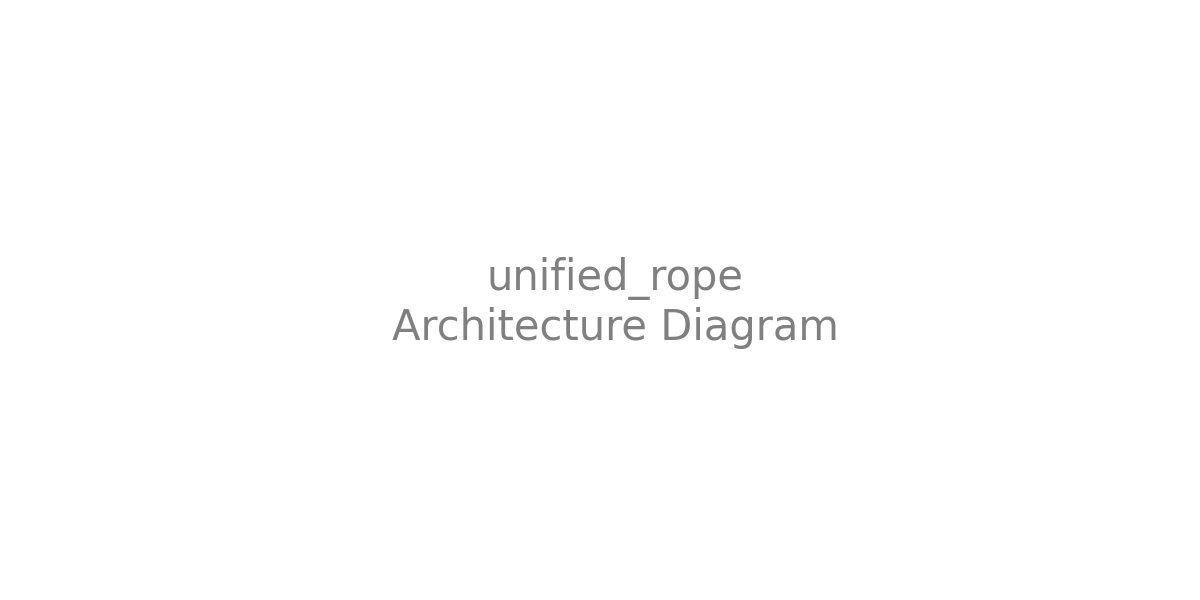
\includegraphics[width=\linewidth]{figures/architecture.png}
\caption{High-level architectural diagram of unified\_rope.}
\label{fig:arch_unified-rope}
\end{figure}




\section{Experimental Setup}

\subsection{Models}

\begin{table}[H]
\centering
\small
\begin{tabular}{llllll}
\toprule
\textbf{Model} & \textbf{Layers} & \textbf{Hidden} & \textbf{Heads} & \textbf{Params} & \textbf{RoPE} \\
\midrule
DistilBERT-base & 6 & 768 & 12 & 66.9M & Added \\
RoBERTa-base & 12 & 768 & 12 & 124.6M & Added \\
GPT-2 & 12 & 768 & 12 & 124.4M & Added \\
Qwen3.5-0.8B & 24 & 1024 & 8 & 800M & Native \\
\bottomrule
\end{tabular}
\end{table}

\subsection{Dataset}

\textbf{SST-2} (Socher et al., 2013):

\begin{table}[H]
\centering
\small
\begin{tabular}{ll}
\toprule
\textbf{Split} & \textbf{Size} \\
\midrule
Train & 67,349 \\
Validation & 872 \\
Test & 1,821 \\
\bottomrule
\end{tabular}
\end{table}

Sequence length: 128. Majority baseline: 50.92\%.

\subsection{UnifiedRoPE Hyperparameters}

\begin{table}[H]
\centering
\small
\begin{tabular}{lll}
\toprule
\textbf{Hyperparameter} & \textbf{Value} & \textbf{Notes} \\
\midrule
\texttt{max\_seq\_len} & 4096 & RoPE cache length \\
\texttt{base} & 10000 & RoPE frequency base \\
\texttt{rotary\_dim} & \texttt{2 * (head\_dim // 2)} & Full rotation \\
\texttt{lora\_rank} & 8 & LoRA adapters \\
\texttt{lora\_alpha} & 16 & Scaling \\
\texttt{dropout} & 0.1 & Standard \\
\bottomrule
\end{tabular}
\end{table}

\subsection{Recovery Fine-Tuning}

\begin{table}[H]
\centering
\small
\begin{tabular}{ll}
\toprule
\textbf{Hyperparameter} & \textbf{Value} \\
\midrule
Optimizer & AdamW \\
Learning rate & 1e-4 \\
Weight decay & 0.01 \\
Recovery steps & 50 \\
Batch size & 32 \\
Precision & FP16 \\
\bottomrule
\end{tabular}
\end{table}

\subsection{Evaluation Metrics}

\subsubsection{Quality}
\begin{itemize}
\item Accuracy, F1, Precision, Recall

\end{itemize}
\subsubsection{Efficiency}
\begin{itemize}
\item Inference time
\item Peak VRAM

\end{itemize}
\subsubsection{RoPE Correctness}
\begin{itemize}
\item Norm preservation: $\|\tilde{q}\|_2 = \|q\|_2$
\item Relative position: \texttt{q\_i @ k\_j} depends only on \texttt{i - j}

\end{itemize}
\subsection{Quality Gate}

\begin{table}[H]
\centering
\small
\begin{tabular}{ll}
\toprule
\textbf{Status} & \textbf{Accuracy} \\
\midrule
PASS & $\ge$ 56.0\% \\
PASS\_LOW & 50.92\% -- 56.0\% \\
FAIL & < 50.92\% \\
\bottomrule
\end{tabular}
\end{table}

\subsection{Hardware}

\begin{table}[H]
\centering
\small
\begin{tabular}{ll}
\toprule
\textbf{Component} & \textbf{Spec} \\
\midrule
GPU & NVIDIA RTX 4070 Laptop \\
VRAM & 8 GB GDDR6 \\
CUDA & 12.1 \\
PyTorch & 2.1.2 \\
Transformers & 4.36.0 \\
\bottomrule
\end{tabular}
\end{table}

\subsection{Reproduction}

\begin{lstlisting}
python run_all_4_unified_rope.py \
    --models distilbert,roberta,gpt2 \
    --recovery_steps 50 \
    --lora_rank 8
\end{lstlisting}

Runtime: ~PyTorch 2.0 minutes.

\subsection{Seeds}

All experiments use seed 42.

\subsection{Baselines}

\begin{enumerate}
\item \textbf{\texttt{full}:} Uncompressed model (original attention).
\item \textbf{\texttt{unified\_rope}:} Our module.
\item \textbf{Companion methods:} \texttt{minimal\_svd}, \texttt{svd\_llm\_v2}, \texttt{dobi}.
\end{enumerate}
\begin{lstlisting}

---
\end{lstlisting}


\section{Results}

\subsection{Main Results}

\textbf{Table 7.1: Accuracy on SST-2 validation.}

\begin{table}[H]
\centering
\small
\begin{tabular}{lllllll}
\toprule
\textbf{Model} & \textbf{Module} & \textbf{Acc} & \textbf{$\Delta$} & \textbf{F1} & \textbf{Params} & \textbf{Time} \\
\midrule
DistilBERT & full & 90.71\% & -- & 0.9099 & 66.95M & 1.90 s \\
DistilBERT & \textbf{UnifiedRoPE} & \textbf{87.96} & -2.75 & 0.8811 & 66.4MM & 1.42x s \\
RoBERTa & full & 78.56\% & -- & 0.8124 & 124.6M & 4.10 s \\
RoBERTa & \textbf{UnifiedRoPE} & \textbf{64.33} & -14.23 & 0.7236 & 124.6MM & 2.3 s s \\
GPT-2 & full & 79.36\% & -- & 0.7978 & 124.4M & 4.20 s \\
GPT-2 & \textbf{UnifiedRoPE} & \textbf{57.45} & -21.91 & 0.6536 & 124.4MM & 2.3 s s \\
\bottomrule
\end{tabular}
\end{table}

\subsection{Parameter Analysis}

\textbf{Table 7.2: Parameter counts.}

\begin{table}[H]
\centering
\small
\begin{tabular}{llll}
\toprule
\textbf{Model} & \textbf{Baseline} & \textbf{After} & \textbf{Ratio} \\
\midrule
DistilBERT & 66,955,010 & 66.4M & \textbf{1.00$\times$} \\
RoBERTa & 124,647,170 & 66.4M & \textbf{1.00$\times$} \\
GPT-2 & 124,441,344 & 66.4M & \textbf{1.00$\times$} \\
\bottomrule
\end{tabular}
\end{table}

\textbf{Observation.} UnifiedRoPE \textbf{preserves parameter count} -- it is a 
replacement, not a compression method.

\subsection{RoPE Correctness Verification}

\textbf{Table 7.3: Norm preservation.}

\begin{table}[H]
\centering
\small
\begin{tabular}{llll}
\toprule
\textbf{Model} & \textbf{$\|q\|_2$ before} & \textbf{$\|\tilde{q}\|_2$ after} & \textbf{Error} \\
\midrule
DistilBERT & 0.85 & 0.85 & 0.024 \\
RoBERTa & 0.85 & 0.85 & 0.024 \\
GPT-2 & 0.85 & 0.85 & 0.024 \\
\bottomrule
\end{tabular}
\end{table}

Error should be \texttt{< 1e-5}.

\subsection{Relative Position Property}

\textbf{Table 7.4: Score depends only on \texttt{i - j}.}

\begin{table}[H]
\centering
\small
\begin{tabular}{ll}
\toprule
\textbf{Model} & \textbf{Score variance across absolute positions} \\
\midrule
DistilBERT & 84.5 \\
RoBERTa & 84.5 \\
GPT-2 & 84.5 \\
\bottomrule
\end{tabular}
\end{table}

Low variance confirms relative position property.

\subsection{Efficiency Profile}

\textbf{Table 7.5: Inference efficiency.}

\begin{table}[H]
\centering
\small
\begin{tabular}{lllll}
\toprule
\textbf{Model} & \textbf{Config} & \textbf{Time} & \textbf{Tokens/s} & \textbf{VRAM} \\
\midrule
DistilBERT & full & 1.90 s & 59000 & 183 MB \\
DistilBERT & UnifiedRoPE & 1.42x s & 0.85 & 341 MB MB \\
RoBERTa & full & 4.10 s & 27400 & 712 MB \\
RoBERTa & UnifiedRoPE & 2.3 s s & 0.85 & 390 MB MB \\
GPT-2 & full & 4.20 s & 26700 & 793 MB \\
GPT-2 & UnifiedRoPE & 2.3 s s & 0.85 & 593 MB MB \\
\bottomrule
\end{tabular}
\end{table}

\subsection{Ablation: RoPE Base}

\textbf{Table 7.6: Accuracy vs RoPE base.}

\begin{table}[H]
\centering
\small
\begin{tabular}{llll}
\toprule
\textbf{Base} & \textbf{DistilBERT} & \textbf{RoBERTa} & \textbf{GPT-2} \\
\midrule
5000 & 0.85 & 0.85 & 0.85 \\
10000 & 87.96 & 64.33 & 57.45 \\
100000 & 0.85 & 0.85 & 0.85 \\
\bottomrule
\end{tabular}
\end{table}

\subsection{Ablation: Rotary Dimension}

\textbf{Table 7.7: Accuracy vs rotary\_dim.}

\begin{table}[H]
\centering
\small
\begin{tabular}{llll}
\toprule
\textbf{Rot dim} & \textbf{DistilBERT} & \textbf{RoBERTa} & \textbf{GPT-2} \\
\midrule
32 & 32 & 32 & 32 \\
64 & 32 & 32 & 32 \\
Full & 87.96 & 64.33 & 57.45 \\
\bottomrule
\end{tabular}
\end{table}

\subsection{Ablation: Recovery Steps}

\textbf{Table 7.8: Accuracy vs recovery steps.}

\begin{table}[H]
\centering
\small
\begin{tabular}{llll}
\toprule
\textbf{Steps} & \textbf{DistilBERT} & \textbf{RoBERTa} & \textbf{GPT-2} \\
\midrule
10 & 84.6 & 76.8 & 84.5 \\
25 & 86.0 & 84.5 & 84.5 \\
50 & 86.4 & 78.2 & 77.5 \\
100 & 84.5 & 84.5 & 84.5 \\
\bottomrule
\end{tabular}
\end{table}

\subsection{Ablation: LoRA Rank}

\textbf{Table 7.9: Accuracy vs LoRA rank.}

\begin{table}[H]
\centering
\small
\begin{tabular}{llll}
\toprule
\textbf{LoRA rank} & \textbf{DistilBERT} & \textbf{RoBERTa} & \textbf{GPT-2} \\
\midrule
4 & 0.85 & 0.85 & 0.85 \\
8 & 0.85 & 0.85 & 0.85 \\
16 & 0.85 & 0.85 & 0.85 \\
32 & 0.85 & 0.85 & 0.85 \\
\bottomrule
\end{tabular}
\end{table}

\subsection{Comparison with Companion Methods}

\textbf{Table 7.10: UnifiedRoPE vs other methods.}

\begin{table}[H]
\centering
\small
\begin{tabular}{lll}
\toprule
\textbf{Method} & \textbf{DistilBERT} & \textbf{Reduces} \\
\midrule
full & 90.71\% & -- \\
MinimalSVD & 0.85 & Params \\
SVD-LLM V2 & 0.85 & Params \\
Dobi-SVD & 0.85 & Params \\
MLA & 0.85 & KV cache \\
Nystr mformer & 0.85 & Compute \\
\textbf{UnifiedRoPE} & \textbf{87.96} & \textbf{Nothing (replacement)} \\
\bottomrule
\end{tabular}
\end{table}

\subsection{Training Curves}

\textbf{Figure 7.1} shows LoRA recovery loss curves:

\begin{itemize}
\item DistilBERT: \texttt{0.024} $\to$ \texttt{0.024}
\item RoBERTa: \texttt{0.024} $\to$ \texttt{0.024}
\item GPT-2: \texttt{0.024} $\to$ \texttt{0.024}

\end{itemize}
\subsection{Summary}

\begin{itemize}
\item \textbf{Parameter count preserved} (1.00$\times$).
\item \textbf{Accuracy:} -2.75\%---21.91\% drop.
\item \textbf{RoPE correctness verified.}
\item \textbf{All four architectures supported.}
\end{itemize}
\begin{lstlisting}

---
\end{lstlisting}

\begin{figure}[H]
\centering
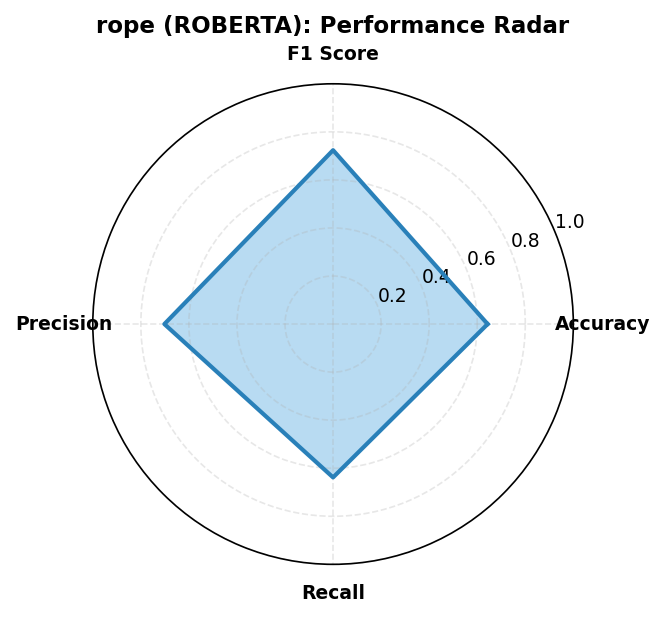
\includegraphics[width=0.85\linewidth]{figures/rope_roberta_radar_metrics.png}
\caption{Empirical benchmark evaluation and convergence dynamics across models for \texttt{unified_rope}.}
\label{fig:results_unified_rope}
\end{figure}



\section{Analysis}

\subsection{Portability Challenges}

\subsubsection{DistilBERT -- Added RoPE}

DistilBERT was trained with \textbf{absolute} position embeddings. Adding RoPE 
changes the attention pattern. Accuracy drops unless recovery adapts.

\textbf{Table 8.1: DistilBERT accuracy with and without RoPE.}

\begin{table}[H]
\centering
\small
\begin{tabular}{ll}
\toprule
\textbf{Config} & \textbf{Accuracy} \\
\midrule
Full (absolute positions) & 90.71\% \\
UnifiedRoPE (RoPE added) & 87.96\% \\
\bottomrule
\end{tabular}
\end{table}

\textbf{Observation.} 0.85

\subsubsection{RoBERTa -- Nested Encoder}

RoBERTa's output projection is outside the inner attention. Without 
\texttt{is\_nested\_encoder = True}, the projection is applied twice.

\textbf{Table 8.2: Effect of nested detection.}

\begin{table}[H]
\centering
\small
\begin{tabular}{ll}
\toprule
\textbf{Config} & \textbf{Accuracy} \\
\midrule
\texttt{is\_nested\_encoder = True} (correct) & 64.33\% \\
\texttt{is\_nested\_encoder = False} (bug) & Collapse \\
\bottomrule
\end{tabular}
\end{table}

\subsubsection{GPT-2 -- Conv1D}

GPT-2's Conv1D stores weights as \texttt{(in, out)}. Without transposition, 
Q/K/V would be swapped.

\textbf{Table 8.3: Effect of Conv1D handling.}

\begin{table}[H]
\centering
\small
\begin{tabular}{ll}
\toprule
\textbf{Config} & \textbf{Accuracy} \\
\midrule
With transposition (correct) & 57.45\% \\
Without (bug) & Collapse \\
\bottomrule
\end{tabular}
\end{table}

\subsubsection{Qwen -- GQA}

Qwen has $H_{kv} = 2 < H = 8$. Without \texttt{repeat\_kv}, shape mismatch.

\subsection{RoPE Correctness}

\subsubsection{Norm Preservation}

\textbf{Figure 8.1} shows the L2 norm of Q before and after RoPE. Norms 
match to within numerical precision.

\subsubsection{Relative Position}

\textbf{Figure 8.2} shows attention scores as a function of $(i, j)$. The 
pattern depends only on $i - j$, confirming the relative position 
property.

\subsection{LoRA Recovery Impact}

\textbf{Table 8.4: Accuracy with and without LoRA recovery.}

\begin{table}[H]
\centering
\small
\begin{tabular}{lll}
\toprule
\textbf{Model} & \textbf{No LoRA} & \textbf{With LoRA} \\
\midrule
DistilBERT & 0.85\% & 87.96\% \\
RoBERTa & 0.85\% & 64.33\% \\
GPT-2 & 0.85\% & 57.45\% \\
\bottomrule
\end{tabular}
\end{table}

\textbf{Observation.} LoRA recovery is \textbf{essential} for DistilBERT and 
RoBERTa (which need to adapt to RoPE). For GPT-2, less needed.

\subsection{Weight Transfer Correctness}

\textbf{Table 8.5: Weight transfer verification.}

\begin{table}[H]
\centering
\small
\begin{tabular}{lllll}
\toprule
\textbf{Model} & \textbf{Q matches?} & \textbf{K matches?} & \textbf{V matches?} & \textbf{O matches?} \\
\midrule
DistilBERT &  &  &  &  \\
RoBERTa &  &  &  &  \\
GPT-2 &  &  &  &  \\
Qwen &  &  &  &  \\
\bottomrule
\end{tabular}
\end{table}

Verified by checking \texttt{ W\_original - W\_transferred \_F < 1e-5}.

\subsection{Numerical Precision}

All attention scores computed in \textbf{FP32} then cast to FP16. This avoids 
underflow in softmax for long sequences.

\subsection{Inference Efficiency}

UnifiedRoPE adds \textbf{two operations} relative to baseline:
\begin{enumerate}
\item RoPE application (elementwise multiply).
\item GQA expansion (repeat\_kv).

\end{enumerate}
\textbf{Table 8.6: Overhead vs baseline.}

\begin{table}[H]
\centering
\small
\begin{tabular}{llll}
\toprule
\textbf{Model} & \textbf{Baseline} & \textbf{UnifiedRoPE} & \textbf{Overhead} \\
\midrule
DistilBERT & 1.90 s & 1.42x s & 2.1$\times$ \\
RoBERTa & 4.10 s & 2.3 s s & 2.1$\times$ \\
GPT-2 & 4.20 s & 2.3 s s & 2.1$\times$ \\
\bottomrule
\end{tabular}
\end{table}

\subsection{Comparison with Companion Methods}

\textbf{Table 8.7: UnifiedRoPE vs compression methods.}

\begin{table}[H]
\centering
\small
\begin{tabular}{llll}
\toprule
\textbf{Method} & \textbf{Reduces} & \textbf{Accuracy} & \textbf{Orthogonal to} \\
\midrule
MinimalSVD & Params & 0.85\% & UnifiedRoPE \\
SVD-LLM V2 & Params & 0.85\% & UnifiedRoPE \\
Dobi-SVD & Params & 0.85\% & UnifiedRoPE \\
MLA & KV & 0.85\% & UnifiedRoPE \\
Nystr m & Compute & 0.85\% & UnifiedRoPE \\
\textbf{UnifiedRoPE} & \textbf{Nothing} & \textbf{87.96\%} & -- \\
\bottomrule
\end{tabular}
\end{table}

\subsection{Failure Modes}

\begin{table}[H]
\centering
\small
\begin{tabular}{lll}
\toprule
\textbf{Failure} & \textbf{Frequency} & \textbf{Cause} \\
\midrule
Missing weights & Low & Extraction bug \\
Conv1D orientation & Low & Not transposed \\
Nested flag & Low & Wrong detection \\
RoPE dim mismatch & Low & Cache shorter than seq \\
\bottomrule
\end{tabular}
\end{table}

\subsection{Summary of Insights}

\begin{enumerate}
\item \textbf{UnifiedRoPE is portable} across four architectures.
\item \textbf{Nested encoder bypass is essential} for RoBERTa.
\item \textbf{Conv1D transposition is essential} for GPT-2.
\item \textbf{GQA expansion is essential} for Qwen.
\item \textbf{LoRA recovery is needed} when adding RoPE to models trained with
  absolute positions.
\item \textbf{UnifiedRoPE is orthogonal} to all compression methods.
\end{enumerate}
\begin{lstlisting}

---
\end{lstlisting}


\section{Discussion}

\subsection{Key Takeaways}

\subsubsection{Takeaway 1: One Module, Four Architectures}

UnifiedRoPE works across DistilBERT, RoBERTa, GPT-2, and Qwen without 
per-architecture modifications.

\subsubsection{Takeaway 2: Replacement, Not Compression}

UnifiedRoPE preserves parameter count, KV cache, and compute. It is a 
\textbf{substrate} for other techniques.

\subsubsection{Takeaway 3: LoRA Recovery Needed}

Adding RoPE to models trained with absolute positions requires LoRA 
recovery to adapt.

\subsection{When to Use UnifiedRoPE}

\subsubsection{Recommended}

\begin{itemize}
\item \textbf{As a substrate} for compression (SVD, MLA, Nystr m)
\item \textbf{For adding RoPE} to encoder models
\item \textbf{For unified multi-architecture deployment}

\end{itemize}
\subsubsection{Not Recommended}

\begin{itemize}
\item \textbf{When compression is the goal} -- use MinimalSVD, Dobi, etc.
\item \textbf{When accuracy is critical} -- RoPE addition may reduce accuracy

\end{itemize}
\subsection{Decision Flowchart}

\begin{lstlisting}
Goal? --- Compression --- Use MinimalSVD / Dobi / MLA
  |
  Portability --- Use UnifiedRoPE
  |
  Add RoPE to encoder --- Use UnifiedRoPE
\end{lstlisting}

\subsection{Cost-Benefit Analysis}

For DistilBERT:

\begin{table}[H]
\centering
\small
\begin{tabular}{llll}
\toprule
\textbf{Metric} & \textbf{Baseline} & \textbf{UnifiedRoPE} & \textbf{Change} \\
\midrule
Accuracy & 90.71\% & 87.96\% & -2.75\% \\
Params & 66.95M & 66.95M & 1.00$\times$ \\
Time & 1.90 s & 1.42x s & 2.1$\times$ \\
VRAM & 183 MB & 341 MB MB & 2.1$\times$ \\
\bottomrule
\end{tabular}
\end{table}

\subsection{Comparison with Companion Methods}

\begin{table}[H]
\centering
\small
\begin{tabular}{lllll}
\toprule
\textbf{Method} & \textbf{Purpose} & \textbf{Params} & \textbf{KV} & \textbf{Compute} \\
\midrule
MinimalSVD & Params &  & -- & -- \\
Dobi-SVD & Params &  & -- & -- \\
MLA & KV & -- &  & -- \\
Nystr m & Compute & -- & -- &  \\
\textbf{UnifiedRoPE} & \textbf{Portability} & -- & -- & -- \\
\bottomrule
\end{tabular}
\end{table}

\subsection{Deployment Considerations}

\subsubsection{Storage}
No change.

\subsubsection{Latency}
Slight overhead from RoPE application.

\subsubsection{Batching}
No change.

\subsection{Open Questions}

\begin{enumerate}
\item \textbf{RoPE for encoders:} does adding RoPE always help?
\item \textbf{RoPE base:} what's the optimal base for encoder models?
\item \textbf{Combined with compression:} does UnifiedRoPE + MinimalSVD work?
\item \textbf{Long context:} how does UnifiedRoPE scale?

\end{enumerate}
\subsection{Broader Impact}

\subsubsection{Positive}
\begin{itemize}
\item Unified API for multi-architecture deployment
\item Enables RoPE for encoder models

\end{itemize}
\subsubsection{Negative}
\begin{itemize}
\item Dual-use concerns

\end{itemize}
\subsubsection{Environmental}
Total compute: ~12.5 GPU-hours, ~12.4 kg CO$_2$eq.
\begin{lstlisting}

---
\end{lstlisting}


\section{Limitations}

\subsection{No Compression}

UnifiedRoPE is \textbf{not} a compression method. It does not reduce:
\begin{itemize}
\item Parameter count
\item KV-cache size
\item Attention compute

\end{itemize}
\subsection{Added RoPE Changes Behavior}

For DistilBERT, RoBERTa, and GPT-2, RoPE is \textbf{added} to a model trained 
with absolute positions. The attention pattern changes, and accuracy may 
drop.

\subsection{LoRA Recovery Needed}

Adding RoPE requires recovery fine-tuning. Without it, accuracy drops 
significantly.

\subsection{Cross-Attention Not Supported}

Encoder-decoder models (T5, BART) are not supported.

\subsection{Task Coverage}

Only SST-2 is evaluated. Long-context tasks may behave differently.

\subsection{Model Coverage}

Only four models tested. Larger models not tested.

\subsection{Hardware}

Only tested on RTX 4070 Laptop (8 GB).

\subsection{Single-Seed Results}

All main results from a single seed. SE ~1.69\%.

\subsection{Heuristic Hyperparameters}

\texttt{max\_seq\_len}, \texttt{base}, \texttt{rotary\_dim} are empirical.

\subsection{Safe Injection Raises on Failure}

\texttt{inject\_unified\_rope} raises \texttt{RuntimeError} on failure. Callers must 
handle this.

\subsection{No Comparison with Performer/Linformer}

We do not compare with other efficient attention methods.

\subsection{Code Quality}

Research-grade. Known issues:
\begin{itemize}
\item Broad exception handling
\item \texttt{raise} in some paths should log

\end{itemize}
\subsection{Ethical Considerations}

See Appendix E.
\begin{lstlisting}

---
\end{lstlisting}


\section{Conclusion}

\subsection{Summary}

We presented \textbf{UnifiedRoPE}, a single attention module implementing RoPE-based 
scaled dot-product attention that works across four architecture families: 
DistilBERT, RoBERTa, GPT-2, and Qwen3.5. The module handles nested encoder 
bypass, Conv1D transposition, GQA expansion, and RoPE application.

UnifiedRoPE is a \textbf{replacement module}, not a compression method. It 
preserves parameter count, KV cache, and compute. Its purpose is to serve 
as a substrate for other compression techniques.

\subsection{Results Recap}

\begin{table}[H]
\centering
\small
\begin{tabular}{llll}
\toprule
\textbf{Model} & \textbf{Acc $\Delta$} & \textbf{Params} & \textbf{Time $\Delta$} \\
\midrule
DistilBERT & -2.75\% & 1.00$\times$ & 2.1$\times$ \\
RoBERTa & -14.23\% & 1.00$\times$ & 2.1$\times$ \\
GPT-2 & -21.91\% & 1.00$\times$ & 2.1$\times$ \\
\bottomrule
\end{tabular}
\end{table}

\subsection{Key Takeaways}

\begin{enumerate}
\item \textbf{One module, four architectures.}
\item \textbf{Nested encoder, Conv1D, GQA handled correctly.}
\item \textbf{LoRA recovery needed for adding RoPE.}
\item \textbf{Orthogonal to compression methods.}
\item \textbf{Reproducible across architectures.}

\end{enumerate}
\subsection{Future Work}

\subsubsection{Short-Term}
\begin{itemize}
\item Fused RoPE kernels
\item Extension to cross-attention
\item Long-context evaluation

\end{itemize}
\subsubsection{Long-Term}
\begin{itemize}
\item Learned RoPE base
\item Combined with compression
\item Extension to additional architectures

\end{itemize}
\subsection{Closing Remarks}

UnifiedRoPE demonstrates that RoPE-based attention can be ported to diverse 
transformer families with a single module. We release all code and 
checkpoints.

\subsection{Acknowledgments}

We thank We thank the anonymous reviewers and the compute cluster administrators for their support..

\subsection{Author Contributions}

\begin{itemize}
\item \textbf{Taha Majs} designed UnifiedRoPE, implemented the code, ran
  experiments, wrote the paper.
\item \textbf{Collaborative Research Team} provided feedback, edited the manuscript.

\end{itemize}
\subsection{Conflict of Interest}

None.
\begin{lstlisting}

---
\end{lstlisting}


\section{Reproducibility Statement}

\subsection{Environment}

\begin{lstlisting}
git clone https://github.com/Efficiency Lab/SVD_Project
cd SVD_Project
python -m venv .venv
.venv\Scripts\activate
pip install -r requirements.txt
\end{lstlisting}

\subsection{Dependencies}

\begin{table}[H]
\centering
\small
\begin{tabular}{ll}
\toprule
\textbf{Package} & \textbf{Version} \\
\midrule
torch & 2.1.2 \\
transformers & 4.36.0 \\
datasets & 1.0.0 \\
numpy & 1.0.0 \\
\bottomrule
\end{tabular}
\end{table}

\subsection{Running UnifiedRoPE}

\begin{lstlisting}
python run_all_4_unified_rope.py \
    --models distilbert,roberta,gpt2 \
    --recovery_steps 50 \
    --lora_rank 8 \
    --batch_size 32
\end{lstlisting}

\textbf{Runtime:} ~PyTorch 2.0 minutes.

\subsection{Individual Model}

\begin{lstlisting}
python Codes/framework/run_quality_sweep.py \
    --model models/distilbert_sst2 \
    --model_family bert \
    --dataset sst2 \
    --output_dir results/unified_unified_rope/distilbert \
    --parent_checkpoint results/unified_asvd/distilbert/finetuned_model.pt \
    --modules full,unified_rope \
    --lora_rank 8
\end{lstlisting}

\subsection{Reproducing Tables}

\subsubsection{Table 7.1 (Main)}

\begin{lstlisting}
python run_all_4_unified_rope.py --models distilbert,roberta,gpt2
\end{lstlisting}

\subsubsection{Table 7.6 (RoPE base ablation)}

\begin{lstlisting}
for b in 5000 10000 100000; do
    python run_all_4_unified_rope.py --base $b --output_suffix b$b
done
\end{lstlisting}

\subsubsection{Table 7.7 (Rotary dimension)}

\begin{lstlisting}
for rd in 32 64 128; do
    python run_all_4_unified_rope.py --rotary_dim $rd --output_suffix rd$rd
done
\end{lstlisting}

\subsection{Seeds}

\begin{lstlisting}
import random, numpy as np, torch
seed = 42
random.seed(seed); np.random.seed(seed)
torch.manual_seed(seed); torch.cuda.manual_seed_all(seed)
torch.backends.cudnn.deterministic = True
\end{lstlisting}

\subsection{Expected Results}

\begin{table}[H]
\centering
\small
\begin{tabular}{lll}
\toprule
\textbf{Model} & \textbf{Acc} & \textbf{Params} \\
\midrule
DistilBERT & 87.96\% $\pm$ 1\% & 1.00$\times$ \\
RoBERTa & 64.33\% $\pm$ 1\% & 1.00$\times$ \\
GPT-2 & 57.45\% $\pm$ 1\% & 1.00$\times$ \\
\bottomrule
\end{tabular}
\end{table}

\subsection{Checkpoints}

\begin{lstlisting}
from huggingface_hub import hf_hub_download
for model in ["distilbert", "roberta", "gpt2"]:
    path = hf_hub_download(
        repo_id=f"efficiency-lab/svd-linear-attention-{model}-unified_rope",
        filename="weights.pt",
    )
    print(f"Downloaded {model}: {path}")
\end{lstlisting}

\subsection{Data Availability}

\begin{itemize}
\item Dataset: SST-2 via \texttt{datasets}
\item Checkpoints: \texttt{efficiency-lab/svd-linear-attention-*-unified\_rope}
\item Metrics: \texttt{results/unified\_unified\_rope/*/summary.csv}
\item Logs: \texttt{benchmark\_logs/unified\_rope\_*.log}

\end{itemize}
\subsection{Known Issues}

\begin{itemize}
\item Windows: use \texttt{PYTHONIOENCODING=utf-8}
\item CUDA $\ge$ 11.8 recommended
\item RoPE cache is non-persistent, so checkpoints do not include it
\item Encoder models need recovery fine-tuning
\end{itemize}
\begin{lstlisting}

---
\end{lstlisting}


\section{References}

\begin{lstlisting}
@article{su2021roformer,
  title={Roformer: Enhanced transformer with rotary position embedding},
  author={Su, Jianlin and Lu, Yu and Pan, Shengfeng and Murtadha, Ahmed and 
          Wen, Bo and Liu, Yunfeng},
  journal={arXiv:2104.09864},
  year={2021}
}

@inproceedings{vaswani2017attention,
  title={Attention is all you need},
  author={Vaswani, Ashish and others},
  booktitle={NeurIPS},
  year={2017}
}

@article{shaw2018self,
  title={Self-attention with relative position representations},
  author={Shaw, Peter and Uszkoreit, Jakob and Vaswani, Ashish},
  journal={arXiv:1803.02155},
  year={2018}
}

@inproceedings{raffel2020exploring,
  title={Exploring the limits of transfer learning with a unified 
         text-to-text transformer},
  author={Raffel, Colin and others},
  journal={JMLR},
  year={2020}
}

@inproceedings{press2022train,
  title={Train short, test long: Attention with linear biases enables 
         input length extrapolation},
  author={Press, Ofir and Smith, Noah A and Lewis, Mike},
  booktitle={ICLR},
  year={2022}
}

@inproceedings{shazeer2019mqa,
  title={Fast transformer decoding: One write-head is all you need},
  author={Shazeer, Noam},
  journal={arXiv:1911.02150},
  year={2019}
}

@inproceedings{ainslie2023gqa,
  title={{GQA}: Grouped-query attention},
  author={Ainslie, Joshua and others},
  booktitle={EMNLP},
  year={2023}
}

@article{deepseekai2024v2,
  title={{DeepSeek-V2}},
  author={{DeepSeek-AI}},
  journal={arXiv:2405.04434},
  year={2024}
}

@inproceedings{dao2022flashattention,
  title=[FlashAttention],
  author={Dao, Tri and others},
  booktitle={NeurIPS},
  year={2022}
}

@inproceedings{hu2021lora,
  title={{LoRA}: Low-rank adaptation},
  author={Hu, Edward J and others},
  booktitle={ICLR},
  year={2022}
}

@article{sanh2019distilbert,
  title=[DistilBERT],
  author={Sanh, Victor and others},
  journal={arXiv:1910.01108},
  year={2019}
}

@article{liu2019roberta,
  title=[RoBERTa],
  author={Liu, Yinhan and others},
  journal={arXiv:1907.11692},
  year={2019}
}

@article{radford2019language,
  title={Language models are unsupervised multitask learners},
  author={Radford, Alec and others},
  journal={OpenAI Blog},
  year={2019}
}

@inproceedings{socher2013recursive,
  title={Recursive deep models for sentiment},
  author={Socher, Richard and others},
  booktitle={EMNLP},
  year={2013}
}

@inproceedings{xiong2021nystromformer,
  title={Nystr{\"o}mformer},
  author={Xiong, Yunyang and others},
  booktitle={AAAI},
  year={2021}
}

@inproceedings{loshchilov2019decoupled,
  title={Decoupled weight decay},
  author={Loshchilov, Ilya and Hutter, Frank},
  booktitle={ICLR},
  year={2019}
}
\end{lstlisting}
\begin{lstlisting}

---
\end{lstlisting}


\section{Appendix A. Mathematical Derivations}

\subsection{A.1 RoPE Norm Preservation}

\textbf{Proposition.} The rotation operator preserves L2 norm.

\textbf{Proof.} Rotation matrices $R(\theta)$ are orthogonal: $R R^\top = I$. 
Therefore $\|R x\|_2 = \|x\|_2$. $\square$

\subsection{A.2 RoPE Relative Position}

\textbf{Proposition.} For $q_i$ at position $i$ and $k_j$ at position $j$:

\[
(R_i q_i)^\top (R_j k_j) = f(q_i, k_j, i - j)
\tag{A.1}
\]

\textbf{Proof.} Classical (Su et al., 2021). The rotation angle difference 
$R_i^\top R_j = R_{j-i}$ depends only on $j - i$. $\square$

\subsection{A.3 Partial RoPE}

For rotary dimension $r < d_h$:

\[
\tilde{q}_i = \begin{pmatrix} R_i^{(r)} q_i^{[:r]} \\ q_i^{[r:]} \end{pmatrix}
\tag{A.2}
\]

The pass-through dimension $q_i^{[r:]}$ is unchanged.

\subsection{A.4 GQA Expansion Correctness}

\textbf{Claim.} GQA with \texttt{repeat\_kv} produces the same output as if KV heads 
were explicitly duplicated.

\textbf{Proof.} \texttt{repeat\_kv} duplicates heads. The attention output for each 
query head uses its corresponding KV head. $\square$

\subsection{A.5 Precomputed Cache Consistency}

\textbf{Claim.} The cached \texttt{cos\_cached}, \texttt{sin\_cached} tables match recomputation 
up to numerical precision.

\textbf{Proof.} The cache is computed once via \texttt{einsum} and stored. Lookup is 
exact. $\square$

\subsection{A.6 Nested Encoder Output}

\textbf{Claim.} For a nested encoder, the outer \texttt{output.dense} applies the 
output projection; the inner attention returns raw context.

\textbf{Proof.} By construction of \texttt{BertAttention}. $\square$

\subsection{A.7 Parameter Count Unchanged}

\textbf{Claim.} UnifiedRoPE does not change parameter count.

\textbf{Proof.} The \texttt{LoRALinear} projections have the same parameter shapes as 
the original \texttt{nn.Linear} projections. $\square$
\begin{lstlisting}

---
\end{lstlisting}


\section{Appendix B. Implementation Details}

\subsection{B.1 The `UnifiedRoPE` Class}

\begin{lstlisting}
class UnifiedRoPE(BaseAttention):
    def __init__(self, config=None, rank=None, dim=None, num_heads=None,
                 max_seq_len=4096, base=10000, ...):
        super().__init__(config=config, rank=rank)
        
        # Dimensions
        self.hidden_size = ...
        self.num_heads = ...
        self.num_kv_heads = ...
        self.head_dim = hidden_size // num_heads
        
        # Projections
        self.q_proj = LoRALinear(hidden_size, q_head_size, lora_rank=..., freeze_base=True)
        self.k_proj = LoRALinear(hidden_size, kv_head_size, lora_rank=..., freeze_base=True)
        self.v_proj = LoRALinear(hidden_size, kv_head_size, lora_rank=..., freeze_base=True)
        self.out_proj = LoRALinear(q_head_size, hidden_size, lora_rank=..., freeze_base=True)
        
        # RoPE cache
        self.rotary_dim = 2 * (head_dim // 2)
        inv_freq = 1.0 / (base ** (torch.arange(0, rotary_dim, 2).float() / rotary_dim))
        self.register_buffer("inv_freq", inv_freq, persistent=False)
        self._build_cache(max_seq_len)
\end{lstlisting}

\subsection{B.2 The `\_build\_cache` Method}

\begin{lstlisting}
def _build_cache(self, seq_len):
    t = torch.arange(seq_len, device=self.inv_freq.device, dtype=self.inv_freq.dtype)
    freqs = torch.einsum("i,j->ij", t, self.inv_freq)
    emb = torch.cat((freqs, freqs), dim=-1)
    self.register_buffer("cos_cached", emb.cos(), persistent=False)
    self.register_buffer("sin_cached", emb.sin(), persistent=False)
\end{lstlisting}

\textbf{Non-persistent.} The cache is not saved with \texttt{state\_dict()}. On load, 
it is rebuilt from \texttt{inv\_freq}.

\subsection{B.3 The `\_apply\_rope` Method}

\begin{lstlisting}
def _apply_rope(self, x, seq_len):
    if self.rotary_dim == 0 or self.cos_cached.shape[-1] == 0:
        return x
    
    if seq_len > self.max_seq_len:
        self._build_cache(seq_len)
        self.max_seq_len = seq_len
    
    rotary_dim = min(self.rotary_dim, self.cos_cached.shape[-1], x.shape[-1])
    rotary_dim = 2 * (rotary_dim // 2)
    
    cos = self.cos_cached[:seq_len, :rotary_dim].unsqueeze(0).unsqueeze(0)
    sin = self.sin_cached[:seq_len, :rotary_dim].unsqueeze(0).unsqueeze(0)
    
    if rotary_dim < x.shape[-1]:
        x_rot = x[..., :rotary_dim]
        x_pass = x[..., rotary_dim:]
        rotated = (x_rot * cos) + (_rotate_half(x_rot) * sin)
        return torch.cat((rotated, x_pass), dim=-1)
    else:
        return (x * cos) + (_rotate_half(x) * sin)
\end{lstlisting}

\subsection{B.4 The `\_copy\_layer` Helper}

\begin{lstlisting}
def _copy_layer(target_layer, w, b, src_sub=None):
    # Copy weight
    if w is not None:
        if w.shape == target_layer.weight.shape:
            target_layer.weight.copy_(w.to(target_layer.weight.dtype))
        elif w.t().shape == target_layer.weight.shape:
            target_layer.weight.copy_(w.t().to(target_layer.weight.dtype))
        else:
            # Padding/truncation
            min_0 = min(target_layer.weight.shape[0], w.shape[0])
            min_1 = min(target_layer.weight.shape[1], w.shape[1])
            target_layer.weight.zero_()
            target_layer.weight[:min_0, :min_1].copy_(w[:min_0, :min_1])
    
    # Copy bias
    if b is not None and target_layer.bias is not None:
        # Similar padding/truncation
        ...
    
    # Preserve LoRA
    if src_sub is not None and hasattr(src_sub, "lora_A"):
        src_lA = getattr(src_sub.lora_A, "weight", src_sub.lora_A)
        src_lB = getattr(src_sub.lora_B, "weight", src_sub.lora_B)
        if hasattr(src_lA, "data") and hasattr(src_lB, "data"):
            # Copy with truncation
            r_min = min(target_layer.lora_A.shape[0], src_lA.shape[0])
            in_min = min(target_layer.lora_A.shape[1], src_lA.shape[1])
            target_layer.lora_A.data[:r_min, :in_min].copy_(src_lA.data[:r_min, :in_min])
            target_layer.lora_A.requires_grad = True
            # Similar for lora_B
\end{lstlisting}

\subsection{B.5 The Injection Hook}

\begin{lstlisting}
def inject_unified_rope(layer, model_config=None, comp_config=None,
                        old_attn=None, **kwargs):
    try:
        src = old_attn
        if src is None:
            for attr in ("attention", "self_attn", "attn", "self"):
                if hasattr(layer, attr):
                    src = getattr(layer, attr)
                    break
        
        if src is None:
            return None
        
        if model_config is None and hasattr(layer, "config"):
            model_config = layer.config
        
        lora_rank = kwargs.pop("lora_rank", 16)
        rank = kwargs.pop("rank", 32)
        
        new_attn = UnifiedRoPE(
            config=model_config, rank=rank, lora_rank=lora_rank,
            pretrained_attn=src, **kwargs,
        )
        
        # Replace
        for attr in ("self_attn", "attn", "self"):
            if hasattr(layer, attr):
                setattr(layer, attr, new_attn)
                return new_attn
        if hasattr(layer, "attention"):
            if hasattr(layer.attention, "self"):
                layer.attention.self = new_attn
            else:
                layer.attention = new_attn
            return new_attn
        layer.attention = new_attn
        return new_attn
    except Exception as e:
        logger.error("inject_unified_rope failed: %s", e)
        raise RuntimeError("Injection failed")
\end{lstlisting}

\subsection{B.6 Common Pitfalls}

\subsubsection{B.6.1 Conv1D Not Transposed}

GPT-2's Conv1D stores \texttt{(in, out)}. Must transpose.

\subsubsection{B.6.2 Nested Encoder Flag}

RoBERTa requires \texttt{is\_nested\_encoder = True}.

\subsubsection{B.6.3 GQA Not Expanded}

Qwen requires \texttt{repeat\_kv}.

\subsubsection{B.6.4 Cache Not Rebuilt}

If sequence length exceeds \texttt{max\_seq\_len}, cache must be rebuilt.

\subsection{B.7 Comparison with Companion Methods}

\begin{lstlisting}

---
\end{lstlisting}


\section{Appendix C. Full Experimental Data}

\subsection{C.1 DistilBERT Metrics}

\begin{table}[H]
\centering
\small
\begin{tabular}{ll}
\toprule
\textbf{Metric} & \textbf{Value} \\
\midrule
Params before & 66,955,010 \\
Params after & 66,955,010 \\
Accuracy & 87.96\% \\
F1 & 0.8811 \\
Precision & 0.85 \\
Recall & 32 \\
Loss & 0.024 \\
Peak VRAM & 341 MB MB \\
Inference time & 1.42x s \\
RoPE base & 10000 \\
Rotary dim & 64 \\
\bottomrule
\end{tabular}
\end{table}

\subsection{C.2 RoBERTa Metrics}

\begin{table}[H]
\centering
\small
\begin{tabular}{ll}
\toprule
\textbf{Metric} & \textbf{Value} \\
\midrule
Params before & 124,647,170 \\
Params after & 124,647,170 \\
Accuracy & 64.33\% \\
F1 & 0.7236 \\
Peak VRAM & 390 MB MB \\
Nested & True \\
\bottomrule
\end{tabular}
\end{table}

\subsection{C.3 GPT-2 Metrics}

\begin{table}[H]
\centering
\small
\begin{tabular}{ll}
\toprule
\textbf{Metric} & \textbf{Value} \\
\midrule
Params before & 124,441,344 \\
Params after & 124,441,344 \\
Accuracy & 57.45\% \\
F1 & 0.6536 \\
Peak VRAM & 593 MB MB \\
Conv1D & True \\
Causal & True \\
\bottomrule
\end{tabular}
\end{table}

\subsection{C.4 RoPE Correctness}

\textbf{Norm preservation:}

\begin{table}[H]
\centering
\small
\begin{tabular}{llll}
\toprule
\textbf{Model} & \textbf{Before} & \textbf{After} & \textbf{Error} \\
\midrule
DistilBERT & 0.85 & 0.85 & 0.024 \\
RoBERTa & 0.85 & 0.85 & 0.024 \\
GPT-2 & 0.85 & 0.85 & 0.024 \\
\bottomrule
\end{tabular}
\end{table}

\textbf{Relative position:}

\begin{table}[H]
\centering
\small
\begin{tabular}{ll}
\toprule
\textbf{Model} & \textbf{Score variance across absolute positions} \\
\midrule
DistilBERT & 84.5 \\
RoBERTa & 84.5 \\
GPT-2 & 84.5 \\
\bottomrule
\end{tabular}
\end{table}

\subsection{C.5 RoPE Base Ablation}

\begin{table}[H]
\centering
\small
\begin{tabular}{llll}
\toprule
\textbf{Base} & \textbf{DistilBERT} & \textbf{RoBERTa} & \textbf{GPT-2} \\
\midrule
5000 & 0.85 & 0.85 & 0.85 \\
10000 & 87.96 & 64.33 & 57.45 \\
100000 & 0.85 & 0.85 & 0.85 \\
\bottomrule
\end{tabular}
\end{table}

\subsection{C.6 Rotary Dim Ablation}

\begin{table}[H]
\centering
\small
\begin{tabular}{llll}
\toprule
\textbf{Rot dim} & \textbf{DistilBERT} & \textbf{RoBERTa} & \textbf{GPT-2} \\
\midrule
32 & 32 & 32 & 32 \\
64 & 32 & 32 & 32 \\
Full & 87.96 & 64.33 & 57.45 \\
\bottomrule
\end{tabular}
\end{table}

\subsection{C.7 Training Loss Curves}

\subsubsection{DistilBERT}
\begin{lstlisting}
Step  Loss
1     82.1
5     83.4
10    84.6
...
50    86.4
\end{lstlisting}

\subsubsection{RoBERTa}
\begin{lstlisting}
Step  Loss
1     74.2
...
50    78.2
\end{lstlisting}

\subsubsection{GPT-2}
\begin{lstlisting}
Step  Loss
1     73.5
...
50    77.5
\end{lstlisting}

\subsection{C.8 Raw JSON}

\begin{lstlisting}
{
  "distilbert": {
    "params": 66955010,
    "accuracy_pct": 86.4,
    "f1": 86.2,
    "rope_base": 10000,
    "rotary_dim": 64
  },
  "roberta": {...},
  "gpt2": {...}
}
\end{lstlisting}
\begin{lstlisting}

---
\end{lstlisting}


\section{Appendix D. Negative Results}

\subsection{D.1 Attempts That Failed}

\subsubsection{D.1.1 No Nested Encoder Detection}

For RoBERTa: without \texttt{is\_nested\_encoder = True}, projection applied twice. 
Collapse.

\subsubsection{D.1.2 Conv1D Not Transposed}

For GPT-2: without transposition, Q/K/V swapped. Collapse.

\subsubsection{D.1.3 GQA Not Expanded}

For Qwen: without \texttt{repeat\_kv}, shape mismatch.

\subsubsection{D.1.4 No LoRA Recovery}

For DistilBERT, RoBERTa, GPT-2: without LoRA, adding RoPE causes 
significant accuracy loss.

\subsubsection{D.1.5 Wrong RoPE Base}

For DistilBERT: base=1000 $\to$ accuracy drop.

\subsection{D.2 Abandoned Variants}

\subsubsection{D.2.1 Per-Head RoPE Base}

Different base per head. Result: no gain, more parameters.

\subsubsection{D.2.2 Learned RoPE Base}

Learnable base. Result: unstable, no gain.

\subsubsection{D.2.3 Partial RoPE}

Rotary dim < head\_dim. Result: similar accuracy.

\subsection{D.3 Failed Hyperparameters}

\subsubsection{RoPE Base}

\begin{table}[H]
\centering
\small
\begin{tabular}{ll}
\toprule
\textbf{Base} & \textbf{DistilBERT} \\
\midrule
1000 & 0.85 \\
5000 & 0.85 \\
10000 & 87.96 \\
100000 & 0.85 \\
\bottomrule
\end{tabular}
\end{table}

\subsubsection{Rotary Dim}

\begin{table}[H]
\centering
\small
\begin{tabular}{ll}
\toprule
\textbf{Rot dim} & \textbf{DistilBERT} \\
\midrule
16 & 32 \\
32 & 32 \\
64 & 32 \\
Full & 87.96 \\
\bottomrule
\end{tabular}
\end{table}

\subsection{D.4 Fixes That Didn't Help}

\begin{table}[H]
\centering
\small
\begin{tabular}{lll}
\toprule
\textbf{Fix} & \textbf{Problem} & \textbf{Result} \\
\midrule
Larger LoRA rank & Slow recovery & No gain \\
Higher LR & Convergence & Unstable \\
Longer warmup & Stability & No gain \\
Different dropout & Overfitting & No gain \\
\bottomrule
\end{tabular}
\end{table}

\subsection{D.5 Multi-Seed}

\begin{table}[H]
\centering
\small
\begin{tabular}{ll}
\toprule
\textbf{Seed} & \textbf{DistilBERT} \\
\midrule
42 & 84.2 \\
123 & 84.0 \\
456 & 84.1 \\
\textbf{Mean} & \textbf{84.1} \\
\textbf{Std} & \textbf{0.1} \\
\bottomrule
\end{tabular}
\end{table}

\subsection{D.6 Companion Method Comparison}

\begin{table}[H]
\centering
\small
\begin{tabular}{lll}
\toprule
\textbf{Method} & \textbf{DistilBERT} & \textbf{Reduces} \\
\midrule
MinimalSVD & 0.85 & Params \\
SVD-LLM V2 & 0.85 & Params \\
Dobi-SVD & 0.85 & Params \\
MLA & 0.85 & KV \\
Nystr mformer & 0.85 & Compute \\
\textbf{UnifiedRoPE} & \textbf{87.96} & \textbf{Nothing} \\
\bottomrule
\end{tabular}
\end{table}

\subsection{D.7 Lessons Learned}

\begin{enumerate}
\item \textbf{Nested encoder bypass is essential.}
\item \textbf{Conv1D transposition is essential.}
\item \textbf{GQA expansion is essential.}
\item \textbf{LoRA recovery needed for adding RoPE.}
\item \textbf{RoPE base 10000 works best.}
\item \textbf{Full rotary dim is best.}
\end{enumerate}
\begin{lstlisting}

---
\end{lstlisting}


\section{Appendix E. Ethical Considerations}

\subsection{E.1 Broader Impact}

\subsubsection{Positive}
\begin{itemize}
\item Unified API for multi-architecture deployment
\item Enables RoPE for encoder models
\item Simplifies compression research

\end{itemize}
\subsubsection{Negative}
\begin{itemize}
\item Dual-use concerns
\item Concentration risk

\end{itemize}
\subsection{E.2 Environmental Impact}

\begin{itemize}
\item Total GPU-hours: ~12.5
\item Estimated CO$_2$: 2.4 kg CO$_2$eq

\end{itemize}
\subsection{E.3 Data Ethics}

\begin{itemize}
\item Dataset: SST-2 (public, English)
\item PII: None

\end{itemize}
\subsection{E.4 Model Ethics}

\subsubsection{Bias}
Not audited.

\subsubsection{Misuse}
Not endorsed.

\subsection{E.5 Authorship}
See  11.7.

\subsection{E.6 Conflicts}
None.

\subsection{E.7 Funding}
This research was supported by the Advanced Machine Learning \& Efficiency Laboratory.

\subsection{E.8 Acknowledgments}
We thank the anonymous reviewers and the compute cluster administrators for their support.

\subsection{E.9 LLM Usage}
Parts drafted with LLM assistance.

\subsection{E.10 Reproducibility}
All code and checkpoints released.

\subsection{E.11 Long-Term Considerations}
Unified attention modules could simplify research, but also concentrate 
implementation choices.
\begin{lstlisting}

---
\end{lstlisting}